\documentclass[border=4pt]{standalone}
% Preámbulo común de las figuras. Cada figura es un documento standalone
% que se compila a SVG con scripts/build_figures.sh
\usepackage[utf8]{inputenc}
\usepackage{amsmath}
\usepackage{tikz}
\usepackage[american, siunitx]{circuitikz}
\usetikzlibrary{arrows.meta,calc,decorations.pathmorphing,patterns}
\tikzset{
  >={Stealth[length=2.2mm]},
  eje/.style={->, thin},
  hilo/.style={thick},
}
% Paleta común: tonos medios legibles sobre fondo claro
\definecolor{azul}{RGB}{31,94,168}
\definecolor{rojo}{RGB}{192,57,43}
\definecolor{verde}{RGB}{39,128,73}
\definecolor{naranja}{RGB}{211,120,30}
\definecolor{morado}{RGB}{125,60,152}

\begin{document}
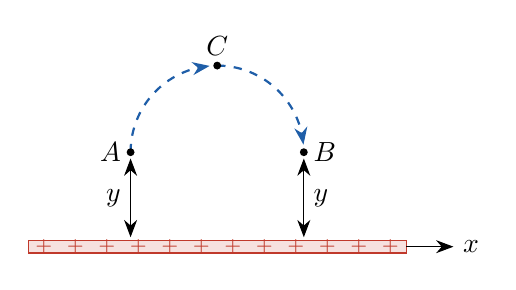
\begin{tikzpicture}[scale=1.0]
  \filldraw[draw=rojo, fill=rojo!15] (-2.4,-0.08) rectangle (2.4,0.08);
  \foreach \x in {-2.2,-1.8,...,2.3} \node[text=rojo, font=\scriptsize, inner sep=0pt] at (\x,0) {$+$};
  \draw[eje] (2.4,0) -- (3.0,0) node[right]{$x$};
  \draw[dashed, thick, azul, ->] (-1.1,1.2) arc (180:95:1.1);
  \draw[dashed, thick, azul, ->] (0,2.3) arc (90:5:1.1);
  \fill (-1.1,1.2) circle (0.05) node[left]{$A$};
  \fill (1.1,1.2) circle (0.05) node[right]{$B$};
  \fill (0,2.3) circle (0.05) node[above]{$C$};
  \draw[<->, thin] (-1.1,0.12) -- node[left]{$y$} (-1.1,1.12);
  \draw[<->, thin] (1.1,0.12) -- node[right]{$y$} (1.1,1.12);
\end{tikzpicture}
\end{document}
